\documentclass[final]{beamer}

\usepackage[scale=1.24]{beamerposter} % Use the beamerposter package for laying out the poster
\usepackage{wrapfig}
\usepackage{subcaption}
\usetheme{confposter} % Use the confposter theme supplied with this template

\setbeamercolor{block title}{fg=ucdblue,bg=white} % Colors of the block titles
\setbeamercolor{block body}{fg=black,bg=white} % Colors of the body of blocks
\setbeamercolor{block alerted title}{fg=ucdgold,bg=ucdblue} % Colors of the highlighted block titles
\setbeamercolor{block alerted body}{fg=black,bg=ucdblue!10} % Colors of the body of highlighted blocks
% Many more colors are available for use in beamerthemeconfposter.sty
\setbeamertemplate{caption}[numbered] 
%-----------------------------------------------------------
% Define the column widths and overall poster size
% To set effective sepwid, onecolwid and twocolwid values, first choose how many columns you want and how much separation you want between columns
% In this template, the separation width chosen is 0.024 of the paper width and a 4-column layout
% onecolwid should therefore be (1-(# of columns+1)*sepwid)/# of columns e.g. (1-(4+1)*0.024)/4 = 0.22
% Set twocolwid to be (2*onecolwid)+sepwid = 0.464
% Set threecolwid to be (3*onecolwid)+2*sepwid = 0.708

\newlength{\sepwid}
\newlength{\onecolwid}
\newlength{\twocolwid}
\newlength{\threecolwid}
\setlength{\paperwidth}{48in} % A0 width: 46.8in
\setlength{\paperheight}{36in} % A0 height: 33.1in
\setlength{\sepwid}{0.012\paperwidth} % Separation width (white space) between columns
\setlength{\onecolwid}{0.22\paperwidth} % Width of one column
\setlength{\twocolwid}{0.464\paperwidth} % Width of two columns
\setlength{\threecolwid}{0.708\paperwidth} % Width of three columns
\setlength{\topmargin}{-0.5in} % Reduce the top margin size
%-----------------------------------------------------------

\usepackage{graphicx}  % Required for including images

\usepackage{booktabs} % Top and bottom rules for tables

\usepackage{subcaption}

\usepackage{natbib}

\usepackage[export]{adjustbox}

% \newenvironment{myitemize}{%
%    \setlength{\topsep}{0pt}
%    \setlength{\partopsep}{0pt}
%    \renewcommand*{\@listi}{\leftmargin\leftmargini \parsep\z@ \topsep\z@ \itemsep\z@}
%    \let\@listI\@listi
%    \itemize
% }{\enditemize}

\setbeamerfont{caption}{size=\small}
%----------------------------------------------------------------------------------------
%	TITLE SECTION 
%----------------------------------------------------------------------------------------

\title{Arctic Mixed-Phase Cloud Dissipation and its Relationship to Low CCN Concentrations} % Poster title

\author{\textbf{Lucas Sterzinger}, Adele L. Igel} % Author(s)

\institute{Atmospheric Science Graduate Group \\ Department of Land, Air, and Water Resources - University of California, Davis} % Institution(s)

%----------------------------------------------------------------------------------------

\begin{document}
%\setbeamercolor{background canvas}{bg=ucdgold!20}
\addtobeamertemplate{block end}{}{\vspace*{2ex}} % White space under blocks
\addtobeamertemplate{block alerted end}{}{\vspace*{2ex}} % White space under highlighted (alert) blocks

\setlength{\belowcaptionskip}{2ex} % White space under figures
\setlength\belowdisplayshortskip{2ex} % White space under equations

\begin{frame}[t] % The whole poster is enclosed in one beamer frame

\begin{columns}[t] % The whole poster consists of three major columns, the second of which is split into two columns twice - the [t] option aligns each column's content to the top

\begin{column}{\sepwid}\end{column} % Empty spacer column

\begin{column}{\onecolwid} % The first column

%----------------------------------------------------------------------------------------
%	OBJECTIVES
%----------------------------------------------------------------------------------------
	\begin{alertblock}{Overview}
		\textbf{Main Question:} Can a lack of environmental CCN/aerosol be a primary factor for Arctic cloud dissipation?
	        \begin{itemize}
            \item Persistent mixed-phase boundary layer clouds are important regulators for Arctic (and global) climate.
            \item Accurately modeling Arctic clouds are important to properly simulate the global climate system.
            \item Unlike in lower latitudes, Arctic aerosol concentrations have been hypothesized to be low enough to inhibit cloud formation
			\begin{itemize}
				\item Mauritsen et al. (2011) coined the term "tenuous clouds" in which cloud structure was limited by aerosol concentration
			\end{itemize}
        \end{itemize}
	\end{alertblock}
	\begin{block}{Cases}
		Two potential cases (Fig. \ref{fig:obs}) have been identified where cloud dissipation occurred coincidentally with a surface aerosol concentration decrease:
		\begin{itemize}
			\item Oliktok Point - May 12th, 2017 - Northern slope of Alaska - ocean/land boundary
			\item ASCOS - August 31st, 2008 - Arctic ocean ice floe
		\end{itemize}
		
\end{block}
\begin{block}{Model Description}
	Regional Atmospheric Modeling System (RAMS) in LES mode. 

	\begin{itemize}
		\item Harrington 2-stream radiation
		\item RAMS 2M bulk microphysics
		\item dx, dy = 62.5 m
		\item dz = 6.25 m
		\item Domain = 6 x 6 x 1.25 km
		\item Cyclic boundary conditions
	\end{itemize}
\end{block}



\end{column} % End of the first column

\begin{column}{\sepwid}\end{column} % Empty spacer column

\begin{column}{\twocolwid}
	% \begin{column}{0.5\linewidth}
		\begin{block}{Case Observations}
			\begin{figure}
				\centering
				\includegraphics[width=0.49\linewidth]{images/oli_timeseries.png}
				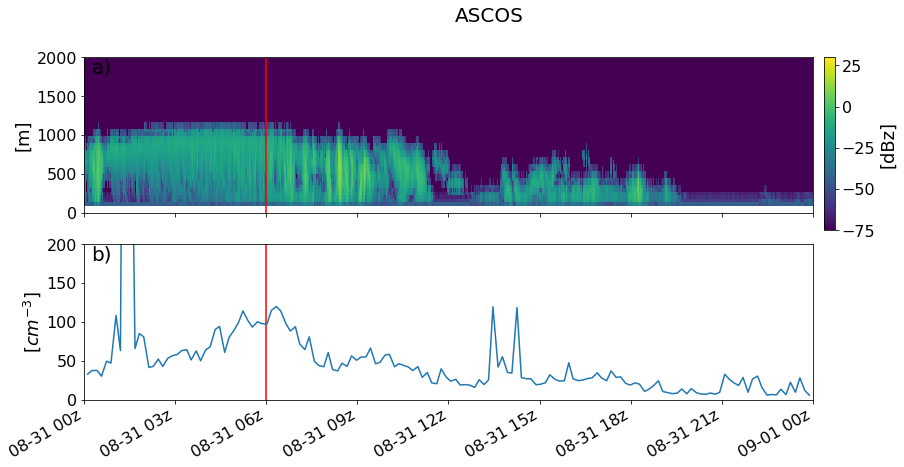
\includegraphics[width=0.49\linewidth]{images/ascos_timeseries.png}
				\caption{Observed Ka-band radar reflectivity (top) and CPC aerosol concentration (bottom) for Oliktok Point and ASCOS}\label{fig:obs}
			\end{figure}	
		\end{block}

	% \end{column}
	% \begin{column}{0.5\linewidth}
	% 	\begin{block}{Initial Profiles}
	% 		\begin{figure}
	% 			\centering
	% 			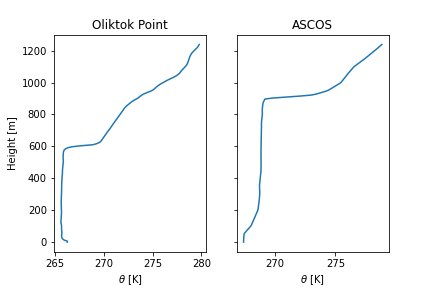
\includegraphics[width=0.9\linewidth]{images/bl_profile.png}
	% 			\caption{Boundary layer $\theta$ profiles used to initialize LES simulations}\label{fig:theta}
	% 		\end{figure}
	% 	\end{block}
	% \end{column}



	\begin{alertblock}{Simulation Results}
		\begin{column}{0.59\linewidth}
			\begin{figure}
				\centering
				\includegraphics[width=\linewidth]{images/oli_lwp.png}
				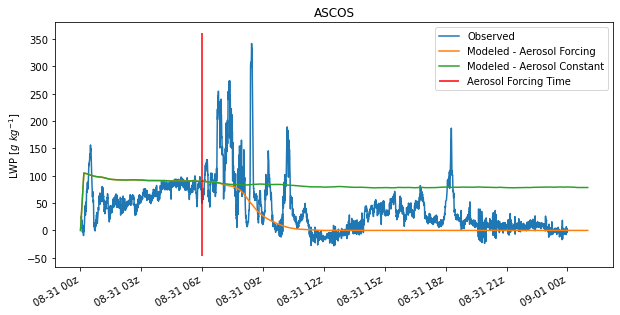
\includegraphics[width=\linewidth]{images/ascos_lwp.png}
				\caption{Observed and simulated liquid water path (LWP) for Oliktok Point (top) and ASCOS (bottom).}\label{fig:simulations}
			\end{figure}
		\end{column}
		\begin{column}{0.5\sepwid}\end{column}
		\begin{column}{0.39\linewidth}
			Balloon soundings (Fig. \ref{fig:theta}) and observed aerosol concentrations used to initialize LES model
			\vspace{1 em}
			
			\underline{Two simulations per case:}
			\begin{itemize}
				\item Stable-cloud control
				\begin{itemize}
					\item Aerosol concentration held constant throughout, no source/sink
				\end{itemize}
				\item Aerosol Forcing Experiment
				\begin{itemize}
					\item Same as control, but aerosol forced to $0\ cm^{-3}$ at the time denoted by the red line
				\end{itemize}
			\end{itemize}
			\vspace{1 em}

			Compare LWP response to aerosol forcing against observed LWP at time of cloud dissipation.
			\begin{itemize}
				\item Oliktok Point simulated LWP response was much slower than observed
				\item ASCOS simulated LWP response was similar to observed
			\end{itemize}
		\end{column}
	\end{alertblock}
\end{column}



\begin{column}{\sepwid}\end{column}

%%%%%%%%%%%%%%
% 3rd column %
%%%%%%%%%%%%%%
\begin{column}{\onecolwid}
	\begin{block}{Discussion}
		The extreme forcing simulations were done to ascertain whether or not aerosol-limited dissipation could be the cause of the observed dissipation cases. These extreme forcing simulations should represent the fastest possible dissipation under a ``tenuous'' regime.

		\begin{itemize}
			\item If the modeled LWP response was slower than the observed, then other effects must be enhancing the dissipation rate
			\item If modeled LWP response was faster than observed, limited aerosol may be the primary cause of dissipation, but is not possible to say for certain
		\end{itemize}
		
	\end{block}
	\begin{alertblock}{Main Takeaways}
		\begin{itemize}
			\item The Oliktok Point simulated LWP response was much slower than observed, indicating that other factors were likely forcing the cloud disspiation	
			\item The ASCOS simulated LWP response matched closely with the observed decay, suggesting that the ASCOS case may have dissipated due to lack of aerosol
		\end{itemize}
	\end{alertblock}
	
	\begin{block}{Conclusions}
		\begin{itemize}
			\item It is difficult to isolate the role of aerosol concentration on observed cloud dissipation
			\item When doing an "extreme" level of aerosol forcing, the ASCOS simulation agreed much closer to observations than Oliktok Point.
			\begin{itemize}
				\item ASCOS dissipation may be forced by aerosol concentrations, but impossible to say for sure
			\end{itemize}
		\end{itemize}
		
		\underline{Future Work}
		\begin{itemize}
			\item Simulate various (and more realistic) aerosol treatment methods
			\item Examine in-cloud processes
			\item Locate and test more cases
		\end{itemize}
		
		
		\small{This work was supported by US Department of Energy Atmospheric System Research Grant \#DE-SC0019073-01}
	\end{block}

\end{column}
\begin{column}{\sepwid}\end{column} % Empty spacer column

\end{columns} % End of all the columns in the poster

\end{frame} % End of the enclosing frame

\end{document}